\chapter{INTRODUÇÃO}

A necessidade de localização no espaço levou a humanidade ao desenvolvimento de diversas ferramentas, tais como os sistemas de coordenadas, a bússola, os mapas, e mais recentemente o Sistema de Posicionamento Global (GPS). Desenvolvido pelos norte americanos se tornou completamente operacional em 1995, com um custo estimado de 10 bilhões de dólares. Consiste de uma constelação de 24 satélites, cada um circulando a Terra duas vezes ao longo do dia, em uma configuração em que ao menos 4 satélites sejam visíveis de qualquer ponto da Terra. O receptor do sinal utiliza a informação enviada pelo satélite para calcular sua distância a cada um destes utilizando a informação entre o instante de recebimento e o instante de transmissão. 

Em 1991, a associação internacional de Aviação Civil utilizou pela primeira vez o termo sistema de navegação por satélite (GNSS - Global Navigation Satellite System), para denominar todo e qualquer sistema semelhante ao GPS, que atualmente é usado para denominar o sistema americano, também conhecido como Navstar GPS. Outro sistema que se encontra completamente operacional é o russo GLONASS. O sistema chinês COMPASS e o europeu GALILEO se encontram em fase de implementação. Considerando a diversidade de sistemas é possível notar sua grande relevância, e como todo sistema está sujeito a pertubações e interferências que devido aos impactos precisam ser estudados, entre elas se pode citar a cintilação ionosférica.

A cintilação ionosférica, medida por meio do índice S4, é definida como o desvio padrão da intensidade do sinal de GPS em um intervalo de um minuto, com 50 amostras por segundo, portanto, quanto maior a pertubação do sinal, maior o valor deste índice. Uma observação que pode ser extraída desta definição, é que dada uma causa para a perturbação do sinal de GPS, é possível que outros sinais de radiofrequência, em regiões relativamente próximas do espectro apresentam interferência semelhante, logo, o índice S4 pode ser interpretado como uma medida de pertubação em sinais de radiofrequência.

Os fenômenos de cintilação, de interesse para este trabalho, decorrem da trajetória do sinal percorrer regiões da ionosfera com baixa densidade de elétrons, com períodos de duração de algumas horas. Estas regiões migram na ionosfera, geralmente no sentido do Sul e do Leste magnético, podendo se expandir ou contrair, sendo denominadas de bolhas ionosféricas. Estas surgem no Hemisfério Sul e sua ocorrência começa a se intensificar de outro a novembro, apresentado picos ao longo do verão, a atividade começa a reduzir em Março. Sua formação começa entre 22:00 UT e 23:00 UT na região do equador magnético, encerrando-se entre as 04:00 e 05:00 UT. Além da atividade mais intensa durante o verão é possível observar uma grande variabilidade dia a dia no decorrer do ano, o que torna difícil sua previsão, \cite{TAKAHASHI:2006}.

A ionosfera, camada de gás da atmosfera ionizada pela radiação solar, é a região onde o fenômeno de interesse se manifesta. Este, assim como outros fenômenos, como a aurora boreal, apresentam um certo nível de organização devido às linhas de campo magnético da Terra. Isto ocorre pois partículas ionizadas ou carregas podem ser mover livremente ao longo das linhas magnéticas mas não entre elas. Assim, o estudo do campo magnético da Terra se faz relevante para um grande número de aplicações, \cite{LAUNDAL:2017}. Um resultado imediato deste estudo é que o norte geográfico e magnético não coincidem, e que simplificadamente o campo magnético poderia ser descrito por um dipolo magnético, com centro comum ao da Terra, porém inclinado em relação a linha que liga o norte e sul geográfico. Atualmente, existe vários sistemas de coordenadas magnéticas cujo proposito dependem da região, da aplicação e da faixa de altitude de interesse, para uma revisão entre os sistemas mais comuns consulte a referência \cite{LAUNDAL:2017}. Para este trabalho foi adotado o sistema AACGM, pois é mais adequado à altura ionosférica, contudo ele pertence a classe de sistemas não-ortogonais.

A ionosfera devido a vários fatores, não somente o campo magnético da Terra, mas toda a interação com o sistema solar, onde o Sol é um dos principais atores, uma vez que é a principal fonte de radiação ionizante, apresenta uma riqueza de fenômenos. Agora, levando em consideração a inclinação do plano de rotação da Terra, em relação ao plano de translação é evidente que em certas regiões há a formação de anomalias. Dentre estas uma de particular interesse, na região Sul, é a anomalia da ionização equatorial que consiste na formação de uma região de alta densidade de elétrons entre 15 e 20 graus de latitude magnética, logo após ao por do Sol. O máximo dessa densidade é denominado de pico da anomalia magnética e se manifesta na região do vale do Paraíba.

Atualmente, não existe um modelo matemático baseado em primeiros princípios, que expresse a física do fenômeno, capaz de modelar e predizer o surgimento e a evolução das bolhas, de forma, que a predição do decorrente fenômeno de cintilação também não é possível. Todavia, os impactos decorrentes desse fenômeno, como a perda de sistemas de navegação, em uma sociedade que apresenta cada vez mais um consumo por este tipo de informação, seja em sistemas de produção como na agricultura \cite{STAFFORD:2000}, ou na aviação, ou para o simples uso pessoal ao percorrer uma cidade, podem ser catastróficas, implicando, por exemplo, em perdas de vidas humanas, ou na redução na produção de alimentos. No caso da aviação, há uma tendência mundial de se utilizar unicamente navegação e procedimentos de pouso/decolagem baseados em GNSS.

Assim, faz-se desejável uma abordagem que permita prever a formação, a evolução das bolhas ionosféricas e intensidade da cintilação dada pelo índice S4. Este índice somente fornece informação indireta sobre a bolha, uma vez que é uma medida da qualidade do sinal de GPS, e este pode sofrer interferências de outras origens. Assim, é necessário uma outra medida quantitativa indicadora de bolhas ionosféricas, o conteúdo eletrônico total vertical (VTEC - Vertical Total Electronic Content), é definido como a quantidade de elétrons, em uma seção vertical de área unitária, cuja unidade de medida é o TECU$=10^{16}$ elétrons/m$^2$. Segundo a literatura, bolhas apresentam valores de VTEC de 30 a 50 TECU inferiores à sua vizinhança.

Na ausência de um modelo que possa simular um fenômeno tão complexo, a alternativa é a utilização de modelos direcionados por dados, isto é, modelos matemáticos que são ajustados para um conjuntos de dados, por exemplo, por processo de optimização. Em um primeiro momento, este termo e sua colocação podem aparecer estranhos, entretanto, eles estão presentes desde o inicio da ciência, um exemplo, são as três leis de Kepler da astronomia, pois estas foram elaboradas por Johannes Kepler extraindo informações de um extenso conjunto de observações catalogadas por Tycho Brahe, ao longo, de sua vida. 

A teoria utilizada para o desenvolvimento desses modelos é vasta, englobando várias áreas da matemática, computação, biologia por meio de algoritmos bio-inspirados. Atualmente, este grande arcabouço teórico e tecnológico se agrupa pelo nome de aprendizado de máquina (machine learning), cuja a ideia básica é o de ajustar uma função, por meio de um mecanismo denominado de aprendizagem, que pode ser, por exemplo, implementado por um método de optimização, a um conjunto de variáveis, atributos. 

Note, que no exemplo citado, tem-se um base de dados, isto é, tipicamente uma grande massa de dados, e um novo conhecimento foi extraído desta. Esse processo, no caso utilizando um algoritmo de aprendizagem, inclui-se no que hoje se chama uma mineração de dados, ou seja, extrair, ou inferir conhecimento novo, que não era evidente a partir do conjunto de dados. A mineração de dados também é adequada para descrever de maneira concisa os dados, classificá-los e predizê-los \cite{HAN:2011}. 

Existem termos que se confundem devido a má utilização, por exemplo, peso e massa, e aqui mineração de dados e descoberta de conhecimento em base de dados, esta é a descoberta de conhecimento, pela extração de padrões representando conhecimento armazenado em um conjunto de dados, enquanto aquela é a extração de padrões em um conjunto de dados. A diferença fica mais clara sumarizando os processos contidos na abordagem de descoberta de conhecimento em base de dados:

A mineração de dados é frequentemente confundida com o processo mais amplo de descoberta de conhecimento em base de dados (KDD- Knowledge Discovery in Databases), a qual é definida como a extração de padrões e desenvolvimento de representações associados ao conhecimento de um processo ou fenômeno a partir de um conjunto de dados associados. A mineração de dados é uma etapa deste processo, a qual é definida como a extração de padrões em um conjunto de dados. As diferenças ficam mais claras as sumarizar-se as etapas contidas em um processo de KDD:

\begin{enumerate}
\item {\bf Limpeza de dados}: remoção de dados com ruído, inconsistentes e incompletos;
\item {\bf Integração de dados}: combinação de múltiplas fontes de dados, por meio de operações como união e intersecção de tabelas;
\item {\bf Seleção de dados}: os dados considerados relevantes ao processo são extraídos do banco de dados;
\item {\bf Transformação de dados}: os dados são transformados e consolidados em uma forma mais apropriada para mineração, sendo por exemplo discretizados, normalizados, agrupados;
\item {\bf Mineração de dados}: é a etapa do KDD associada com a aplicação de algoritmos estatísticos, de reconhecimento de padrões ou de inteligência computacional (caso dos algoritmos de aprendizado de máquina), como por exemplo, redes neurais, árvores de decisão, visando a extração de padrões;
\item {\bf Avaliação de padrões}: avaliação dos modelos desenvolvidos, por exemplo, medir o desempenho de um sistema de classificação;
\item {\bf Apresentação do conhecimento}: técnicas de visualização e representação dos dados são usadas para exibir o conhecimento extraído aos usuários.
\end{enumerate} 

O processo de KDD é iterativo, como pode ser visto na figura \ref{fig:kdd} no sentido em que etapas podem ser revistas e reexecutadas em função dos resultados obtidos. Além disso, seu passos e a ordem destes podem variar conforme o autor. Por exemplo, neste trabalho, é feita um pré-seleção dos dados, seguido de um pré-processamento que envolve interpolação e suavização, e então uma seleção mais refinada dos dados.

\begin{figure}[H]
\centering
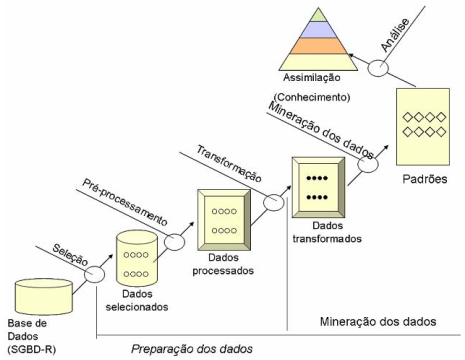
\includegraphics[width=0.8\columnwidth]{./Figuras/kdd.png}
\label{fig:kdd}
\caption{Passos de um processo de KDD. Fonte: Rezende, F. L. C. (2009)}
\end{figure}

Os algoritmos de mineração de dados podem ser agrupados em dois grandes grupos: os supervisionados e os não-supervisionados. Na última década apareceram variações, tais como, algoritmos autosupervisionados, ou semisupervisionados. Seja $\mathcal{X}$ o domínio dos atributos, ou exemplos, e $\mathcal{Y}$ o domínio dos rótulos, um algoritmo é dito supervisionado quando busca uma função $f : \mathcal{X} \to \mathcal{Y}$, tal que $f(\textbf{x})$ consiga predizer o rótulo $y$ correto para uma dada observação $\textbf{x}$, a partir de um conjunto de treino $\{(x_i, y_i)\}_{i=1}^n$ \cite{ZHU:2009}.

A classificação e a regressão, são dois exemplos de algorítimos supervisionados que visam predizer as saídas lidando com valores discretos e contínuos, respectivamente. Algoritmos não supervisionados, por sua vez, são utilizados quando se deseja encontrar algum padrão na estrutura do conjunto de dados. Comumente métodos como, clusterização, detecção de novidade e redução da dimensionalidade são aplicados neste tipo de paradigma, onde o conjunto de treino $\{x_i\}_{i=1}^n$ não diz nada a respeito sobre os rótulos de cada observação.

Considerando-se um escopo mais ambicioso, de predição da ocorrência de cintilação, o objetivo deste trabalho restringe-se à utilização de técnicas de mineração e visualização de dados históricos da ionosfera, de forma a analisar a evolução espaço-temporal do índice S4 e do TEC e sua correlação. Este trabalho objetiva complementar trabalhos anteriores relacionados à predição da ocorrência de cintilação \cite{REZENDE:2009, GLAUSTON:2014, GLAUSTON:2015}, além de trabalhos relacionados ao objetivo específico aqui abordado, como por exemplo a correlação entre o gradiente do TEC e a cintilação \cite{RAGHAVARAO:1998, RAY:2006}, ou então a correlação entre a derivada temporal do TEC e a cintilação \cite{RAGHUNATH:2016}.

Os dados utilizados neste trabalho se restringem ao período de atividade solar máxima de um ciclo solar, no caso, de 01/12/2013 até 28/02/2014. Devido a problemas técnicos e de equipamentos/sensores, existem muitas lacunas nestes dados, exigindo cuidados especiais no seu processamento.
